\subsection{Antennenoszillator}\label{subsec:Antennenoszilator}
Für die Antennenoszillator Schaltung übernahmen wir die bereits im Projekt 5 eingesetzte Colpitts-Oszillator Schaltung. Die aus dem P5 übernommene Schaltung ist in Abbildung bla \todo{Schaltung} gezeigt. 

Die Schaltung ist eine Colpitts-Oszillator Schaltung mit einem JFET. 
Damit das Sinussignal des Antennenoszillator nicht A/D gewandelt werden muss, wurde entschieden das Sinussignal in ein Rechtecksignal mit gleicher Frequenz zu wandeln. Dies geschieht mithilfe einer Komparatorschaltung. 

Wie in Abbildung \ref{img:Schema} zu sehen ist wird das PCB mit \SI{12}{V} und \SI{3.3}{V} DC betrieben. Diese Spannungen werden von Labornetzgeräten erzeugt. Um die Versorgungsspannung zu stabilisieren wurden für beide Spannungen ein  \SI{100}{nF} Keramikkondensator und ein \SI{10}{uF} Elektrolytkondensator verbaut. 
Der Colpitts-Oszillator wird wie im Franzis Bauset mit \SI{12}{V} DC betrieben. Dies ist nötig um ein genügend starkes elektrisches Feld der Antenne zu erzeugen. Im Versuchsaufbau wurde versucht den Colpitts-Oszillator mit \SI{3.3}{V} zu betreiben. Mit \SI{3.3}{V} ist jedoch das elektrische Feld der Antenne zu klein. Der Spieler kann nur sehr nahe an der Antennen das elektrische Feld beeinflussen.
Die Komparatorschaltung wird mit \SI{3.3}{V} betrieben da die Logikeingänge des FPGA auf diese Spannung ausgelegt sind, und das Signal \textit{osc\_out} diesen Pegel haben muss.

Als Antenne wird ein Messingrohr verwendet. Dieses ist zwischen der Spule L1 und dem Kondensator C1 verbunden. 
Da der im Bauset verwendete JFET nicht mehr bestellbar ist, wurde der J113 N-Channel JFET verwendet. Die mit LTspice simulierten Werte des J113 glichen stark der original Schaltung, weshalb dieser gewählt wurde. 

\begin{figure}[h]
	\centering
	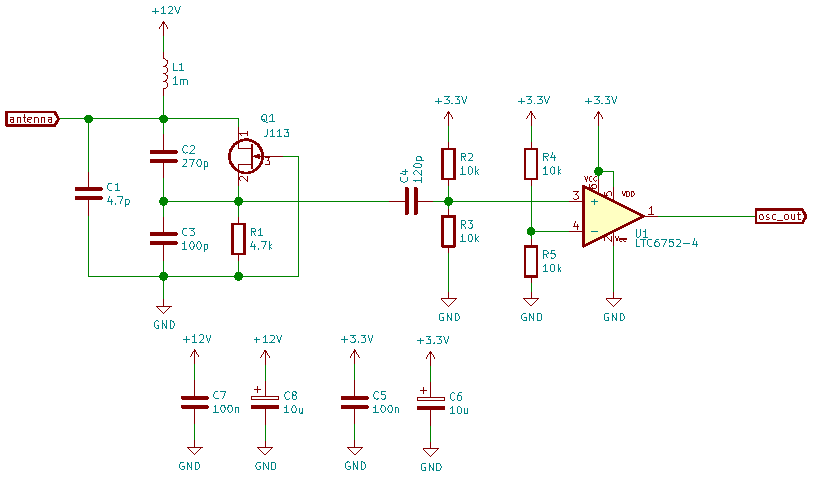
\includegraphics[width=0.9\textwidth]{Schema.pdf}
	\caption{ Schema Antennenoszillator. Links Collpitts-Oszillator,rechts Komparatorschaltung}
	\label{img:Schema}
\end{figure}

\clearpage

Die Ausgangsspannung des Colpitts-Oszillator wird über den Kondensator C4 entkoppelt. Dabei wird der DC-Anteil entfernt. Der Kondensator C4 und die Widerstände R2 und R3 bilden zusammen einen Hochpass. Damit die Oszillator Frequenz von ca \SI{570}{kHz} das Filter passieren kann wurde C4 so gewählt das die Grenzfrequenz des Filters bei ca \SI{265}{kHz} liegt. 

Um das Sinussignal des Colpitts-Oszillators in ein Rechtecksignal zu wandeln wurde eine nichtinvertierende Komparatorschaltung gewählt. Dazu wurde der LTC6752 Komparator mit Rail to Rail und Single Supply verwendet \cite{LTC}. Als Referenzspannung wurde die halbe Versorgungsspannung gewählt. Diese wurde mit den Widerständen R4 und R5 realisiert.


